\chapter{My Project}

\section{Project's purpose}\label{condition}

\textbf{Electronic Tourist Refund Scheme} (ETRS) is a government's project, which allowed the tourists who visit Singapore could reclaim Good and Service Tax if he bought a product in Singapore.

To be able to reclaim the refund money, a condition have to be satisfied: 
\begin{itemize}
	\item receipt's value must exceed 100 SGD
	\item merchant or shop who generated the receipt must registry for the ETRS project
	\item if receipt's value don't exceed 100 SGD, it could be grouped with maximum another 2 receipts, such that the total value of this group must exceed 100 SGD and all the receipts within this group must belong to the same merchant or shop
\end{itemize}



Our job is to realize the idea of the ETRS project into mobile device. 

\section{Important technics implemented}

\subsection{BlinkID}
BlinkID is a library allow scanning the passport of tourist. From the information we got from the scan, we can create account for the tourist, thus each person is associated with his/her passport. So even if a tourist lost his account, the refund process still could going on if he still keep his passport.

The mechanic of the scanning is that it will read the \textbf{Machine Readable Zone} (MRZ). 

\begin{figure}
\centering
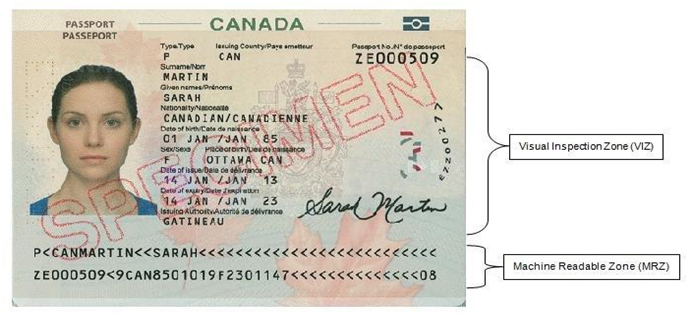
\includegraphics[scale=0.7]{passport_mrz}
\caption{Passport with MRZ zone}
\end{figure}

\subsection{QR code}
Each tourist, after registry their account, is given 1 QR code. In case that he don't want to show his passport, he could use this QR code to identify himself. Each merchant or shop would have their own QR code, and the tourist can scan their QR code for the ID of the shop. 

In this project, I've implemented the scanning and generating QR code using a library, created by JourneyApps.
\begin{itemize}
	\item website: \href{http://journeyapps.com/}{http://journeyapps.com/}
	\item github:\href{https://github.com/journeyapps/zxing-android-embedded}{ https://github.com/journeyapps/zxing-android-embedded}
\end{itemize}

\subsection{Android location service}
Using this service, the application will notice the tourist if he's near one of the shop registry for the ETRS project. This service locates the user's position either by wifi or by GPS.

\subsection{Geofencing}
This function allow the application to detect if the user is going in or out of the airport, thus allow to take correspondant behavior.

\subsection{Push notification}
This allows the server to notify users when there're changes in their data, such as if their request to refund is realized, or refused. 

\subsection{Google Cloud Message (GCM)}
The application allow user to define their events that need to be notified when the time come, for example the flight's time. Application will use GCM to notify the user when such time come.

\subsection{Social network sharing}
The application allow user to share on their social network, such as Facebook, Wechat, Sina Weibo. And this is abig challenge, because China's social network (Wechat, Sina Weibo) do not have many tutorials in English, and the procedure to register application ID on these network is complicated too. 

\subsection{Map}
Google Map service is intergrated into the application, thanks to the need of path finder. It's not very complicated, but then the problem rise. As Google Map can't be used inside China, we have to adopt another map service from China, Baidu map, and this process is extremely difficult, from the registration process to implementation process, since this service only work if you are in China, even fake GPS couldn't help.

\subsection{Communication method between client and server}
We mainly use RestAPI, since it's lightweight, and easy to implement. For security purpose, we generate for each user each times they login an \textbf{user-token}. Each time a client want to make a request, the user-token will be included into header of request. Beside, base on this user-token, we could identify user, and prevent the client from spamming request to server.

The response is under form of \textbf{JSON} format. And since Google have greatly supported JSON, parsing a JSON response into Java model is plain easy.  


\section{Algorithm utilized}

I was given the task to write the algorithm that filter a list of receipts and return receipts which satisfy the condition in  \ref{condition}. 

\subsection{Brief description}
Given the list of receipts, could be generated by many shops, extract a list of receipts which satisfy the conditions in \ref{condition}.

\subsection{Solution}
We devide the list of receipts into many lists such that the receipts in each list belong to one shop only. This lead to a new problem: 
Given the list of receipts, all receipts belong to 1 shop, extract a list of receipts which satisfy the condition in \ref{condition}

\subsubsection{Step 1}
Extract all the receipts which value greater or equal 100. Then sort the rest of list in increased order.

\subsubsection{Step 2}
Divide the ordered list into many smaller lists :

\begin{algorithm}[H]
\caption{Split list of receipts into many sublists}
\begin{algorithmic}[1]
\Function{SplitList}{receipts}
\State $j = 0, i = 0$
\While{$i < \textit{receipts}.length$}
\If {$\Big[ \cfrac{\textit{receipts}[i].value}{10} \Big]  \leq  j$}
	\State $list_{j}.add(\textit{receipts}[i])$
	\State $i++$.
\Else
	\State $j++$
\EndIf
\EndWhile
\EndFunction
\end{algorithmic}
\end{algorithm}

\subsubsection{Step 3}
From the sublists, we will extract groups of receipts which satisfy the condition. There's some preconditions we could make for simplifier the process.

\begin{itemize}
\item for a group of 2 receipts, if they belong to $list_{i}$ and $list_{j}$ then $i+j \geq 9$
\item for a group of 3 receipts, if the belong to $list_{i}$, $list_{j}$ and $list_{k}$ then $i+j+k \geq 8$
\end{itemize}


First of all we need a function that check the condition of a set of receipt. If satisfy, remove the receipts from their correspondant sublist, and add a new group of receipt to our list of group and return true. Otherwise return false.

\begin{algorithm}[H]
\caption{Check if the correspondant receipts could form a group}
\begin{algorithmic}[1]
\Function{Check}{i, j, k, a, b, c, groups}

\State $r_{a} = list_{i}[a]$
\State $r_{b} = list_{j}[b]$
\State $r_{c} = list_{k}[c]$

\If{$r_{a}.value + r_{b}.value \geq 100 \land (i \neq j \lor a \neq b)$}
	\State groups.add(\textbf{new} Group($r_a, r_b$))
	\State $list_i.remove(r_a), list_j.remove(r_b)$
	\State \Return{true}
\EndIf

\If{$r_{b}.value + r_{c}.value \geq 100 \land (j \neq k \lor b \neq c$}
	\State groups.add(\textbf{new} Group($r_b, r_c$))
	\State $list_j.remove(r_b), list_k.remove(r_c)$
	\State \Return{true}
\EndIf

\If{$r_{a}.value + r_{c}.value \geq 100 \land (i \neq k \lor a \neq c)$}
	\State groups.add(\textbf{new} Group($r_a, r_c$))
	\State $list_i.remove(r_a), list_k.remove(r_c)$
	\State \Return{true}
\EndIf

\If{$r_a.value + r_b.value + r_c.value \geq 100 \land (i \neq j \lor a \neq b) \land (i \neq k \lor a \neq c) \land (j \neq k \lor b \neq c)$}
	\State groups.add(\textbf{new} Group($r_a, r_b, r_c$))
	\State $list_i.remove(r_a), list_j.remove(r_b), list_k.remove(r_c)$
	\State \Return{true}
\EndIf

\Return{false}
\EndFunction
\end{algorithmic}
\end{algorithm}

The next function is the main one that extract a list of groups of receipts from the sublists.

\begin{algorithm}[H]
\caption{}
\begin{algorithmic}[1]
\Function{Filter}{}
\State $i=0, j=0, k=0$
\State groups
\State \underline{loop\_i}:
\For{$i=0$ \textbf{to} $9$}
	\State $a=b=c=0$
	\While{$a < list_i.size$}
	\State \underline{loop\_j}:
	\For{$j=i$ \textbf{to} $9$}
		\State $b=c=0$
		\While{$b < list_j.size$}
		\State \underline{loop\_k}:
		\For{$k=j$ \textbf{to} $9$}
			\State $c=0$
			\While{$a < list_i.size \land b < list_j.size \land c < list_k.size$}
				\If{$i=j$}
					\If{$a=b$}
						\If{$i+k \geq 9$}
							\If{$j \neq k \lor a \neq c$}
								\If{$\neg \Call{Check}{i,j,k,a,b,c,groups}$}
									\State $c++$
								\EndIf
							\Else
								\State $c++$
							\EndIf
						\Else
							\State \textbf{goto} \underline{loop\_k}
						\EndIf
					\Else % a!=b AND i=j
						\If{$k=j \land (c=a \lor c=b)$}
							\If{$i+j \geq 9$}
								\If{$\neg \Call{Check}{i,j,k,a,b,c,groups}$}
									\State $c++$
								\EndIf
							\Else
								\State \textbf{goto} \underline{loop\_k}
							\EndIf						
						\Else
							\If{$\neg \Call{Check}{i,j,k,a,b,c,groups}$}
								\State $c++$
							\EndIf
						\EndIf
					\EndIf
				\Else % i!=j break into page 2 here
				\algstore{filterbreak}
				\end{algorithmic}
				\end{algorithm}
				
\clearpage

				\begin{algorithm}
				\begin{algorithmic}
				\algrestore{filterbreak}
					\If{$j=k$}
						\If{$b=c$}
							\If{$\neg \Call{Check}{i,j,k,a,b,c,groups}$}
								\State $c++$
							\EndIf
						\Else
							\If{$i+j+k \geq 8$}
								\If{$\neg \Call{Check}{i,j,k,a,b,c,groups}$}
									\State $c++$
								\EndIf
							\Else
								\State \textbf{goto} \underline{loop\_k}
							\EndIf
						\EndIf
					\Else % j!=k
						\If{$i+j+k \geq 8$}
							\If{$\neg \Call{Check}{i,j,k,a,b,c,groups}$}
								\State $c++$
							\EndIf
						\Else
							\State \textbf{goto} \underline{loop\_k}
						\EndIf
					\EndIf
				\EndIf
			\EndWhile
		\EndFor
		\State $b++$
		\EndWhile
	\EndFor
	\State $a++$

	\EndWhile
\EndFor
\State \Return{groups}
\EndFunction
\end{algorithmic}
\end{algorithm}


At this stage we get a list which consists of :
\begin{itemize}
	\item receipts which are greater than 100
	\item groups of receipts, maximum 3 receipts, which are greater than 100
\end{itemize}

Repeat for all lists of receipts of different merchant or shop, and we got the solution.